%%%%%%%%%%%%%%%%%%%%%%%%%%%%%%%%%%%%%%%%%%%%%%%%%%%%%%%%%%%%%%%%%%%%%%%%%%%%%%%%
%2345678901234567890123456789012345678901234567890123456789012345678901234567890
%        1         2         3         4         5         6         7         8

\documentclass[letterpaper, 10 pt, conference]{ieeeconf}  % Comment this line out
                                                          % if you need a4paper
%\documentclass[a4paper, 10pt, conference]{ieeeconf}      % Use this line for a4
                                                          % paper

\IEEEoverridecommandlockouts                              % This command is only
                                                          % needed if you want to
                                                          % use the \thanks command
\overrideIEEEmargins
% See the \addtolength command later in the file to balance the column lengths
% on the last page of the document

\usepackage[final]{graphicx}
\usepackage[text={7in,10in},centering,top=72pt,bottom=54pt,right=54pt,left=54pt]{geometry}
\usepackage{color}
\usepackage{amsmath}
\usepackage{amssymb}
\usepackage[linesnumbered,ruled]{algorithm2e}
\usepackage{amsfonts}
\usepackage{hyperref}
\usepackage{float}
\usepackage{caption}
% \usepackage[numbers,sort&compress]{natbib}
\usepackage{tikz}
% \usepackage{setspace} % Double spacing
% %\doublespacing
\pdfminorversion=4
\usepackage{subcaption}
\usepackage{cite}
\hypersetup{
    bookmarks=true,         % show bookmarks bar?
    unicode=false,          % non-Latin characters in Acrobat’s bookmarks
    pdftoolbar=true,        % show Acrobat’s toolbar?
    pdfmenubar=true,        % show Acrobat’s menu?
    pdffitwindow=false,     % window fit to page when opened
    pdfstartview={FitH},    % fits the width of the page to the window
    pdftitle={Robust Fault Detection in Distributed Positive Systems},    % title
    pdfauthor={Sam Nazari},     % author
    pdfsubject={Robust Fault Detection},   % subject of the document
    pdfcreator={Sam Nazari},   % creator of the document
    pdfproducer={Sam Nazari}, % producer of the document
    pdfkeywords={Fault Detection} 
                {Graph Algorithms} 
                {Robust Observer} 
                {Graph Laplacian}, % list of keywords
    pdfnewwindow=true,      % links in new PDF window
    colorlinks=false,       % false: boxed links; true: colored links
    linkcolor=red,          % color of internal links (change box color with linkbordercolor)
    citecolor=green,        % color of links to bibliography
    filecolor=magenta,      % color of file links
    urlcolor=cyan           % color of external links
}

\newtheorem{theorem}{Theorem}
\newtheorem{corollary}{Corollary}
\newtheorem{lemma}{Lemma}
\newtheorem{prop}{Proposition}
%\theoremstyle{definition}
\newtheorem{definition}{Definition}
\newtheorem{example}[theorem]{Example}
\newtheorem{xca}[theorem]{Exercise}
\newtheorem{app}{Application}
\newtheorem{ass}{Assumption}
\newtheorem{cond}{Condition}
\newtheorem{problem}{Problem}

%\theoremstyle{remark}
\newtheorem{remark}{Remark}

%  \numberwithin{equation}{section}

%    Absolute value notation
\newcommand{\abs}[1]{\lvert#1\rvert}

%    Circled numbers
\newcommand*\circled[1]{\tikz[baseline=(char.base)]{
            \node[shape=circle,draw,inner sep=2pt] (char) {#1};}}
            
%    Blank box placeholder for figures (to avoid requiring any
%    particular graphics capabilities for printing this document).
\newcommand{\blankbox}[2]{%
  \parbox{\columnwidth}{\centering
%    Set fboxsep to 0 so that the actual size of the box will match the
%    given measurements more closely.
    \setlength{\fboxsep}{0pt}%
    \fbox{\raisebox{0pt}[#2]{\hspace{#1}}}%
  }%
}

\sloppy
\definecolor{lightgray}{gray}{0.5}
\setlength{\parindent}{0pt}

%  Some of my shortcuts 

\def\X{b}
\def\tX{\tilde{b}}
\def\mX{B}
\def\tmX{\tilde{B}}
\def\bone{{\bf 1}}
\def\bzero{{\bf 0}}
\def\bx{{\bf x}}
\def\by{{\bf y}}
\def\bz{{\bf z}}
\def\bof{{\bf f}}
\def\N{\mathbb{N}}
\def\Z{\mathbb{Z}}
\def\Q{\mathbb{Q}}
\def\R{\mathbb{R}}
\def\Rp{\mathbb{R}_+}
\def\Rpp{\mathbb{R}_{++}}
\def\tT{\mathsf{T}} % Transpose
\def\C{\mathbb{C}}
\def\mP{\mathbb{P}}
\def\mE{\mathbb{E}}
\def\mI{\mathbb{I}}
\def\mM{\mathbb{M}}
\def\cA{\mathcal{A}}
\def\cN{\mathcal{N}}
\def\cV{\mathcal{V}}
\def\cE{\mathcal{E}}
\def\cC{\mathcal{C}}
\def\cT{\mathcal{T}}
\def\cS{\mathcal{S}}
\def\cP{\mathcal{P}}
\def\cB{\mathcal{B}}
\def\cG{\mathcal{G}}
\def\cL{\mathcal{L}}
\def\cVGD{\mathcal{V}_{G_d}}
\def\cEGD{\mathcal{E}_{G_d}}
\def\cVHD{\mathcal{V}_{H_d}}
\def\cEHD{\mathcal{E}_{H_d}}
\def\eps{\epsilon}
\def\reff{\textup{Reff}}
\def\deg{\textup{deg}}
\def\GD{G_d=(\cVGD,\cEGD)}
\def\HD{H_d=(\cVHD,\cEHD)}
\def\gez{\geq 0}
\def\gz{>0}
\def\lez{\leq 0}
\def\lz{<0}
\newcommand{\etal}{\textit{et al}. }
\newcommand{\ie}{\textit{i}.\textit{e}., }
\newcommand{\eg}{\textit{e}.\textit{g}. }

\DeclareMathOperator*{\argmax}{\arg\!\max}

% The following packages can be found on http:\\www.ctan.org
%\usepackage{graphics} % for pdf, bitmapped graphics files
%\usepackage{epsfig} % for postscript graphics files
%\usepackage{mathptmx} % assumes new font selection scheme installed
%\usepackage{times} % assumes new font selection scheme installed
%\usepackage{amsmath} % assumes amsmath package installed
%\usepackage{amssymb}  % assumes amsmath package installed

\title{\Large \bf
Positive Unknown Input Observer for Fault Detection of Positive Distributed Systems}
%Robust Fault Detection in Distributed Systems
%\author{ \parbox{3 in}{\centering Huibert Kwakernaak*
%         \thanks{*Use the $\backslash$thanks command to put information here}\\
%         Faculty of Electrical Engineering, Mathematics and Computer Science\\
%         University of Twente\\
%         7500 AE Enschede, The Netherlands\\
%         {\tt\small h.kwakernaak@autsubmit.com}}
%         \hspace*{ 0.5 in}
%         \parbox{3 in}{ \centering Pradeep Misra**
%         \thanks{**The footnote marks may be inserted manually}\\
%        Department of Electrical Engineering \\
%         Wright State University\\
%         Dayton, OH 45435, USA\\
%         {\tt\small pmisra@cs.wright.edu}}
%}

\author{\parbox{7 in}{\centering Sam Nazari and Bahram Shafai \\
%         \thanks{*Use the $\backslash$thanks command to put information here}\\
          Department of Electrical Engineering, Northeastern University, Boston MA\\ nazari@ece.neu.edu
%         7500 AE Enschede, The Netherlands\\
%         {\tt\small h.kwakernaak@autsubmit.com}}
%         \hspace*{ 0.5 in}
%         \parbox{3 in}{ \centering Pradeep Misra**
%         \thanks{**The footnote marks may be inserted manually}\\
%        Department of Electrical Engineering \\
%         Wright State University\\
%         Dayton, OH 45435, USA\\
%         {\tt\small pmisra@cs.wright.edu}}
}}%Sam Nazari, Bahram Shafai}
\begin{document}
\maketitle
\thispagestyle{empty}
\pagestyle{empty}


%%%%%%%%%%%%%%%%%%%%%%%%%%%%%%%%%%%%%%%%%%%%%%%%%%%%%%%%%%%%%%%%%%%%%%%%%%%%%%%%
\begin{abstract}
We consider robust fault detection in distributed systems with first and second order agent models. In such systems, we show that a ubiquitous class of consensus protocols leads to collective dynamics that lie in a nonnegative invariant set. Based on this, we derive LMI conditions for residual generators to sense faults in the nonnegative invariant set. An illustrative example is provided to highlight our approach and to show that it can reduce the time interval between fault occurrence and fault detection. 
\end{abstract}

%%%%%%%%%%%%%%%%%%%%%%%%%%%%%%%%%%%%%%%%%%%%%%%%%%%%%%%%%%%%%%%%%%%%%%%%%%%%%%%%
\section{Introduction} \label{sec:intro}
Society relies on large, complex systems that are fundamentally networked \cite{wolf_safety_2018,nazari_distributed_2016}. Many of these systems constitute the critical infrastructures that modernity depends on. Typically, these complex infrastructures are made up of smaller subsystems, sometimes called agents, that interact locally with neighbors through information pathways.  Examples of these infrastructures include financial transaction networks, information bearing networks, and energy production networks \cite{pasqualetti_control-theoretic_2015}. A distributed system is a system wherein such agents interactions are constrained to a local set of neighboring agents. 

It is well known that the design of distributed systems is a multidisciplinary endeavor. Currently, there is major emphasis on development of rigorous design tools in order to assist system architecture planners in designing networked control systems (NCS) and Cyber-Physical Systems (CPS) \cite{teixeira_attack_2012,pasqualetti_control-theoretic_2015}. To address these demands, investigators have recently approached the design of distributed systems from a system theoretic perspective \cite{pasqualetti_control-theoretic_2015}. In particular linear observers have been formulated to address a variety of  problems (delay, robust, singular, positive) \cite{oreilly_observers_1983,shafai_proportional-integral_2015} as well as a variety of applications (fault detection, cyberphysical security, etc) \cite{chen_robust_1999,teixeira_distributed_2014}. 

Due to its robust disturbance decoupling properties, the Unknown Input Observer (UIO) plays a central role in the analysis and design of observers for systems subject to unknown disturbance inputs \cite{p._kudva_n._viswanadham_a._ramakrishna_observers_1980,m._hou_p._muller_design_1992}. Recently, the authors of \cite{shafai_positive_2015} reported the conditions that must be satisfied in order to design a positive UIO (PUIO) for a positive linear dynamical systems in terms of LMIs. This development is important since many physical systems may be modeled as positive linear systems \cite{farina_positive_2000,kaczorek_positive_2002,berman_nonnegative_1989}. In the distributed setting, however, no equivalent results have been reported in the literature.  Furthermore, distributed systems are frequently plagued by actuator and sensor faults. If such faults are not adequately addressed, they may lead to biases in the overall consensus solution of the network or unexpected system behavior.  Consequently, there is a growing need to formulate positive observers for distributed positive systems. 

\medskip

To that end, fault detection in distributed systems has received notable attention from researchers recently. In \cite{teixeira_distributed_2017}, the authors address the problem of distributed reconfiguration of networked control systems.  Various decentralized observer structures are surveyed in \cite{shafai_proportional-integral_2015} for fault detection in distributed systems. In \cite{teixeira_distributed_2014} and \cite{shames_distributed_2012} the authors consider distributed fault detection and isolation with imprecise network models. The authors of \cite{terelius_consensus_2013} consider the consensus dynamics of a specific fault that leads to positive feedback in the distributed system. 

Many of the distributed systems that are addressed by the aforementioned approaches can be classified as positive linear systems. A positive linear system is a linear system whose state trajectories are confined to lie in the positive orthant \cite{farina_positive_2000,kaczorek_positive_2002,berman_nonnegative_1989,dautrebande_positive_1999,shafai_robust_2016}. Fault detection for such systems involves designing residual generators with internally positive state observers. In this paper we show that two popular linear consensus protocols lead to collective dynamics that can naturally be modeled as positive linear systems. After establishing this, we introduce distributed positive unknown input observers (D-PUIOs) using an LMI formulation to robustly estimate the states of individual agents, decoupled from unknown external disturbances, so that they can be processed by a residual generator to sense faults in distributed topologies. In doing this, we address the problem of designing positive residual generators to sense faults in a networked or distributed system with first or second order agent dynamics that are confined to the nonnegative orthant using an LMI formulation. 

Section \ref{sec:back} provides background on systems theory, section \ref{sec:PUIO} introduces PUIO and show how to formulate PUIO based residual generators, section \ref{sec:DPUIO} shows that the distributed systems in this paper are positive systems and the D-PUIO for robust residual generation is introduced. An illustrative example is provided in Section \ref{sec:Example} with concluding remarks in Section \ref{sec:con}.

\section{Background} \label{sec:back}
\subsection{Notation}
We denote the set of all positive real numbers including zero with the symbol $\Rp = \{x \in \R: x\geq 0\}$. %Note that $\Rp$ forms an additive semigroup $(\Rp, +)$ and a multiplicative group $(\Rp, \times)$ with 1 as the natural element. 
%The set $\theta x$ with $\theta \geq 0$ and $x \in \Rp$ forms a cone, denoted by $\mathcal{K}$. A cone $\mathcal{K}$ is a proper cone if it is convex, closed, solid and pointed \cite{boyd_convex_2004}. The nonnegative orthant forms a proper cone which we denote by $\mathcal{K}^n$. 
For convenience, nonnegative matrices are denoted by $M \geq 0$. We use similar notation for vectors and scalars. Relatedly, we use the notation $M > 0$ to mean the matrix $M$ with entries that are strictly positive. We reserve the symbol $\succeq$ refer to positive semi-definite matrices, \eg $P \succeq 0$. 
Graph theory has proven to be useful in a variety of diverse applications. We denote a graph by $\cG = (\mathcal{V},\mathcal{E})$. We assume all graphs are simple, finite, and undirected.  The set of \textit{neighbors} of the vertex $v \in \mathcal{V}$ is denoted by $\mathcal{N}_v$. The notation $|\mathcal{N}_v|=m$ denotes the cardinality of the set of neighbors of $v$, in this case $m$. 
\subsection{Positive Systems}
Consider the general linear, time invariant system
\begin{gather}\label{eq: xdot}
\begin{aligned} 
\dot{x}(t) &= Ax(t) + Bu(t) + Ef(t)  \\
y(t) &= Cx(t) + Du(t)
\end{aligned}
\end{gather}
where $x \in \mathbb{R}^n$, $u \in \mathbb{R}^m$, $y \in \mathbb{R}^p$, $f \in \mathbb{R}^r$ are state, input, output and fault vectors, respectively, and $A \in \mathbb{R}^{n \times n}$, $B \in \mathbb{R}^{n \times m}$, $C \in \mathbb{R}^{p \times n}$, $D \in \mathbb{R}^{p \times m}$ and $E \in \mathbb{R}^{n \times r}$ are associated system matrices. Let us further assume the system is in minimal representation meaning that the pair $\{A,B\}$ and $\{A,C\}$ are controllable and observable respectively. Note that the following definitions and lemmas are standard and can be found in \cite{farina_positive_2000}. 
%The following definition is a slight generalization of the well known definition of positive systems and the subsequent results are standard \cite{Berm89,Kac2002,Far2000}.

\begin{definition} \label{def:Metz}
A general linear system with initial condition $x_0 \gez$ is said to be internally positive if $u(t), \hspace{1mm} f(t) \gez$ implies $x(t), \hspace{1mm} y(t) \gez \hspace{1mm}\forall t \gez$.
\end{definition}

\begin{definition} A matrix $A = [a_{ij}] \in \mathbb{R}^{n \times n}$ is called a Metzler matrix if all of its off-diagonal elements are nonnegative, \ie $a_{ij} \geq 0, \forall i \neq j,\hspace{2mm} i,j = 1, \ldots , n$.  
\end{definition}

\begin{remark} \label{rem:rem1}
Furthermore, a Metzler matrix is called strictly Metzler if in addition the condition in definition \ref{def:Metz} we have $a_{ii} < 0$ $\forall i = 1,\ldots,n$. 
\end{remark}

\begin{remark}
Throughout the paper, we shall denote the space of Metzler matrices with the symbol $\mM$.
\end{remark}

\begin{remark}
Every Metzler matrix $A$ has a real eigenvalue $\mu = \lambda_{max} (A) = \max \text{Re}{(\lambda_i)}$ $ \forall i = 1, \ldots,n$ and a corresponding eigenvector $v_{max} \geq 0$. If $\mu < 0$ then $\text{Re}{(\lambda_i)} < 0$ $\forall i = 1,\ldots,n$ where $\lambda_i$ are the eigenvalues of $A$ \cite{berman_nonnegative_1989,farina_positive_2000}.
\end{remark}

%A positive system may also possess an important property known as \textit{reducibility}. %Formally, we have the following definition.

\begin{definition}
A positive system is said to be \textit{reducible} if and only if the free evolution of a set of $n_1$ state variables is independent of the free evolution of the remaining $n_2 = n - n_1$ state variables. A system that is not reducible is said to be \textit{irreducible}.
\end{definition}

\begin{lemma} \label{lem:lemIntPos}
The system in (\ref{eq: xdot}) is internally positive if and only if $A \in \mM$ and $B \gez$, $C \gez$, and $E \gez$.  
\end{lemma}

%\begin{lemma} \label{lem:lemma2}
%Let the system (\ref{eq: xdot}) be internally positive. Then it is asymptotically stable if and only if one of the following equivalent conditions is satisfied:
%\begin{enumerate}
%\setlength\itemsep{2mm}
%\item All eigenvalues of the $A$ have negative real parts.
%\item All coefficients of the characteristic polynomial 
%\begin{align*}
%det(\lambda I - A) = \lambda^n + a_{n-1} \lambda^{n-1}+ \ldots +a_1 \lambda + a_0
%\end{align*}
%are positive, \ie $a_i > 0$ $\forall i = 0,1,\ldots n-1$.
%\item All leading principal minors of $-A$ are positive.
%\item The matrix $A$ is nonsingular and $-A^{-1} > 0$.
%\item There exists a positive definite (possibly diagonal) matrix $P$ such that $A^T P + PA \prec 0$.
%\item There exists a vector $v \in \mathbb{R}_+^n$ such that $Av < 0$.
%\end{enumerate}
%\end{lemma}
\begin{lemma} \label{lem:3}
A positive system $(A,B,E,C)$ is irreducible if and only if its influence graph $\cG$ is connected, or, equivalently, if and only if 
\begin{align}
I + \cA +\cA^2 + \ldots + \cA^{n-1} \nonumber
\end{align}
is a strictly positive matrix, where $\cA$ is the adjacency matrix of $\cG$.
\end{lemma}
%Furthermore, an irreducible positive system may be cyclic or primitive. A cyclic irreducible positive system arises when the set of state variables can be partitioned into classes such that every variable in class $C_i$ has a direct influence only on variables of the ensuing classes, \ie $C_{i+1}$ for $i = 1,2,\ldots r-1$ and every variable in class $C_r$ has a direct influence only on variables of the class $C_1$. Irreducible positive systems that do not hold this property are said to be \textit{primitive}. %This motivates the following result. 
% \begin{lemma}
% An irreducible positive system $(A,B,C,E)$ is primitive if and only if the greatest common divisor $M$ of the length of all the simple cycles in its influence graph $\cG$ is 1. Otherwise, the system is cyclic and its cyclicity index r is equal to $M$. 
% \end{lemma}
% \subsubsection{Positive Dynamic Systems}
% \subsubsection{Positive Observers}
% \subsubsection{Robustness In Observer Theory}
\subsection{Distributed Systems}
% \textcolor{red}{Note that: $L \in \mathbb{R}^{n \times n}$, $x \in \mathbb{R}^n$, $y \in \mathbb{R}^m$, $C_i \in \mathbb{R}^{m\times n}$, $b_j \in \mathbb{R}^n$, $D_i \in \mathbb{R}^{n \times m}$ and that $|\mathcal{N}_i| = k$.}
\subsubsection{First-Order Dynamics} Consider a group of $n$ agents with state $\psi_i(t)$ having single integrator dynamics 
\begin{gather} 
\begin{aligned}
\dot{\psi}_i(t) &= u_i(t), \nonumber \\
y_i(t) &= \psi_i (t) \nonumber
\end{aligned}
\end{gather}
starting with initial condition $\psi_i (0) = \psi_{i0} \in \R$. The underlying interactions of such a interconnected system can be modeled by an undirected graph, $\cG = (\mathcal{V},\mathcal{E})$. Let the first-order consensus law 
$u_i(t) = \sum_{j \in \mathcal{N}_i} (\psi_j(t) - \psi_i(t))$
be assumed; where $u_i(t)$ is the control input to agent $i \in \mathcal{V}$, $x_i(t) \in \mathbb{R}$ is the state of agent $i$ and $\psi_j(t) \in \mathbb{R}$ is the state of one of agent $i$'s neighbors. In the case where there are no faults or disturbances, the model 
\begin{gather} 
\begin{aligned} \label{eq:agentCons}
\dot{\psi}_i(t) &= \sum_{j \in \mathcal{N}_i} (\psi_j(t) - \psi_i(t)) \\
y_i(t) &= \psi_i(t) \nonumber
\end{aligned}
\end{gather}
is valid for each agent $i \in \mathcal{V}$. Under these assumptions, the collective dynamics of the entire network are given by \cite{olfati-saber_consensus_2007}:
\begin{align} \label{eq:consensysDynSingle}
\dot{\mathbf{x}}(t) = -\cL\mathbf{x}(t)
\end{align}
where $\cL \in \mathbb{R}^{n \times n}$ is the graph Laplacian of $\cG$ and $\mathbf{x}(t) \in \mathbb{R}^n$ is the state vector. In a distributed system, each agent $i \in \mathcal{V}$ only has access to the states of the $m$ agents in its local neighborhood, $\mathcal{N}_i$. Let the set of states available to agent $i \in \mathcal{V}$ be defined by:
%\begin{align} %\label{eq:Ci}
$w_i(t) = \left [ \begin{array}{ccc} \psi(t)_{i_1},&\ldots,&\psi(t)_{i_{|\mathcal{N}_i}|} \end{array}\right ]^{\tT} = C_i \mathbf{x}(t)$ %\nonumber
%\end{align}
where $C_i \in \mathbb{R}^{m \times n}$ encodes the interconnection topology of agent $i \in \mathcal{V}$. 
In the presence of faults, the system model for the agent that is subject to the fault must be modified since it no longer updates its state according to the consensus protocol. Instead, if agent $j \in \mathcal{N}_i$ experiences an fault, then it may update its state according to:
\begin{gather} 
\begin{aligned} %\label{eq:agentConsFaultAct}
\dot{\psi}_j(t) &= \sum_{i \in \mathcal{N}_j} (\psi_i(t) - \psi_j(t))+f_j(t) \nonumber \\
y_j(t) &= \psi_j(t)
\end{aligned}
\end{gather}
where $f_j(t)$ is a function of time that is due to the fault signal. The network dynamics become \cite{teixeira_toward_2014}:
\begin{gather} \label{eq:globalDynActFaultSingle}
\begin{aligned} 
\dot{\mathbf{x}}(t) &= -\cL\mathbf{x}(t)+Ef(t) \\
\mathbf{y}(t) &= \mathbf{x}(t)
\end{aligned}
\end{gather}
 where $E \in \mathbb{R}^{n \times r}$ is the fault distribution matrix. %If, instead, agent $j$ is 
\subsubsection{Second-Order Dynamics}
Consider a group of $n$ agents with state $x(t)=\left [\psi(t) \hspace{1mm} \omega (t) \right]^{\tT}$ having double integrator dynamics 
\begin{gather} \label{eq:doubleInt}
\begin{aligned}
\dot{\psi}_i(t) &= \omega_i(t), \\
\dot{\omega}_i(t) &= u_i(t) + v_i(t) \nonumber
\end{aligned}
\end{gather}
with $v_i(t)$ being a known external input and $u_i(t)$ given by the linear consensus protocol 
\begin{align}
u_i(t) = & -\kappa_i \omega_i(t) \nonumber \\
		 &  +\sum_{j \in \mathcal{N}_i} w_{ij} \left [ (\psi_j(t) - \psi_i(t)) + \gamma (\omega_j(t) - \omega_i(t)) \right ] \nonumber
\end{align}
where $w_{ij} > 0$ is the edge weight and $\kappa_i, \gamma \geq 0$ for $i, j = 1, \ldots, n$ are scalar coefficients.  The subscript $i$ and $j$ denote the agent and its neighbor, respectively.  The collective dynamics of the distributed system are then modeled by \cite{ren_distributed_2007,teixeira_toward_2014}
\begin{gather}  \label{eq:doubleCons}
\begin{aligned}
\dot{\mathbf{x}}(t) &= A_{\cG} \mathbf{x}(t) + Bv(t) \\
\mathbf{y}(t) &= \mathbf{x}(t)
\end{aligned}
\end{gather}
where 
\begin{align} \label{eq:AB}
A_{\cG} = \left [\begin{array}{cc}
0 & I \\
-\cL & -\gamma \cL -\bar{K}
\end{array} \right ], \hspace{2mm} B = \left [ \begin{array}{c} 0 \\ I \end{array} \right]
\end{align}
where $\cL \in \R^{2n \times 2n}$ is the graph Laplacian of $\cG$ and $\bar{K} = diag(\kappa_1, \ldots, \kappa_n)$. In the presence of faults, the system model for the agent that is subject to the fault must be modified since it no longer updates its state according to the consensus protocol. Instead, if agent $j \in \mathcal{N}_i$ experiences a fault, then it may update its state according to $\dot{\psi}_j(t) = \omega_j (t) + f_j (t)$, or, if the fault is imparted on the second state variable 
\begin{gather} 
\begin{aligned} \label{eq:agentConsFaultAct}
\dot{\psi}_j(t) &= \omega_j(t) \\
\dot{\omega}_j (t) &= u_j (t) + v_j (t) +f_j (t) \nonumber
\end{aligned}
\end{gather}
where $f_j$(t) is a function of time that is due to the fault signal. The network dynamics become:
\begin{gather} \label{eq:globalDynActFault}
\begin{aligned} 
\dot{\mathbf{x}}(t) &= A_{\cG}\mathbf{x}(t)+Bv(t)+Ef(t) \\
\mathbf{y}(t) &= \mathbf{x}(t).
\end{aligned}
\end{gather}

%%%%%%%%%%%%%%%%%%%%%%%%%%%%%%%%%%%%%%%%%%%%%%%%%%%%%%%%%%%%%%%%%%%%%%%%%%%%%%%%
\section{Positive Unknown Input Observers For Fault Detection \& Isolation} \label{sec:PUIO}
\subsection{Positive Unknown Input Observer Structure}
An unknown input observer for the system in (\ref{eq: xdot}) has the following structure
\begin{align} \label{eq:UIO}
\dot{z}(t) &= Fz(t) +Gy(t) +Hu(t) \\ 
\hat{x}(t) &= Mz(t) + Ny(t). \nonumber
\end{align}
For simplicity we assume $M=I$, $G = G_1 + G_2$ and $H=TB$. In fault detection and isolation, residual signals are processed in order to determine if a fault has occurred. Based on the PUIO in (\ref{eq:UIO}), the residual generator is given by
\begin{align}
r (t) &= (I - C H ) y (t) - C z (t). \label{eq:residual}
\end{align} 
Related to (\ref{eq:UIO}) we have the following lemma.
\begin{lemma} \label{lem:lemmaUIO}
The UIO (\ref{eq:UIO}) is an internally positive unknown input observer if and only if $F \in \mM$, $G \gez$, $H\gez$, $N \gez$ and $u(t) \gez$ implies that $z(t) \gez, \hat{x}(t) \gez, y(t) \gez, \hspace{1mm} \forall t\geq 0$. 
\end{lemma}
\begin{proof}
This is a consequence of definition (\ref{def:Metz}) and lemma (\ref{lem:lemIntPos}).
\end{proof}
\subsection{Generalized Inverse of a Nonnegative Matrix}
The generalized inverse of a nonnegative matrix is needed to design a PUIO. The Moore-Penrose generalized inverse of $\widetilde{A} \in \R^{m \times n}$ is the unique matrix $\widetilde{A}^g \in \R^{m \times n}$, satisfying the equalities $(i)$ $\widetilde{A}^g = \widetilde{A}^g \widetilde{A} \widetilde{A}^g$, $(ii) \widetilde{A}= \widetilde{A} \widetilde{A}^g \widetilde{A}$, $(iii) (\widetilde{A} \widetilde{A}^g)^T = \widetilde{A} \widetilde{A}^g$, and $(\widetilde{A}^g \widetilde{A})^T = \widetilde{A}^g \widetilde{A}$. %We refer the interested reader to any matrix analysis book for details and assume the requisite mathematical background for the remainder of the paper. 

In general the existence of $\widetilde{A} \gez$ does not imply $\widetilde{A}^g \gez$. For $\widetilde{A} \gez$ square and invertable we have $\widetilde{A}^g = \widetilde{A}^{-1} \geq 0$ iff $\widetilde{A}$ is monomial. A monomial matrix is a generalized permutation matrix. %\ie there exists exactly one nonzero entry in each row and the same for each column.  
We can express a monomial matrix as a product of a diagonal matrix and permutation matrix. Similarly, its inverse can be expressed as $\widetilde{A}^{-1} = D\widetilde{A}^T$ for some diagonal matrix $D$ with positive diagonal elements.  Our goal is to provide the necessary and sufficient conditions on $\widetilde{A} \geq 0$ so that $\widetilde{A}^g \geq 0$. To accomplish this, we use the following result from \cite{berman_nonnegative_1989} which characterizes $\widetilde{A} \geq 0$ so that $\widetilde{A}^g \geq 0$. 

\begin{lemma} \label{lem:pinvP}
Let $\widetilde{A} \gez$ with rank $r$.  Then the following statements are equivalent:
\begin{enumerate}
\item $\widetilde{A}^g \gez$.
\item There exists a permutation matrix $\widetilde{P}$ such that $\widetilde{P}\widetilde{A}$ has the form $\widetilde{P}\widetilde{A} = \left [ \widetilde{B_1}^T\ldots\hspace{1mm}\widetilde{B_r}^T  0 \right ]^T$,
% \begin{align*}
% \widetilde{P}\widetilde{A} = \left [ \begin{array}{c} \widetilde{B_1} \\ \vdots \\ \widetilde{B_r} \\ 0 \end{array} \right ]
% \end{align*}
where each $\widetilde{B_i}$ has rank 1 and the rows of $\widetilde{B_i}$ are orthogonal to the rows of $\widetilde{B_j}$ for $i \neq j$.
\item $\widetilde{A}^g = D \widetilde{A}^T$ for some diagonal matrix $D$ with positive diagonal elements.
\end{enumerate}
\end{lemma}

The interested reader may find the proof of lemma \ref{lem:pinvP} in \cite{berman_nonnegative_1989} We now construct $\widetilde{A}^g$.  Under statement 2 in lemma \ref{lem:pinvP}, we let $\widetilde{B}= \widetilde{P}\widetilde{A}$.  Then $\forall i = 1 \ldots r, \hspace{2mm}$ there exist column vectors $x_i , y_i$ such that $\widetilde{B_i}=x_i y_i^T$. Furthermore, $\widetilde{B_i}^g$ is the nonnegative matrix
%\begin{align*}
$\widetilde{B_i}^g = (||x_i||^2 ||y_i||^2)^{-1} \widetilde{B_i}^T$
%\end{align*}
and moreover $\widetilde{B}^g = (\widetilde{B_1}^g, \ldots , \widetilde{B_r}^g, 0)$, since $\widetilde{B_i} \widetilde{B_j}=0$ for $i \neq j$. In particular, $\widetilde{B}^g = D \widetilde{B}^T$ where $D$ is a diagonal matrix with positive diagonal elements and thus $\widetilde{A}^g = D \widetilde{A}^T$.
\subsection{Design of PUIO Based Residual Generators}
The following result is important in designing PUIOs that can be used to produce residual signals for fault detection in positive dynamic systems. 
\begin{theorem} \label{thrm:altPUIO}
Consider a positive system defined by (\ref{eq: xdot}) with the fault term $f(t) \neq 0$ such that $rank(CE) = rank(E) = r$ and the generalized left inverse of $CE$ is nonnegative. Then there exists a PUIO of the form (\ref{eq:UIO}) if and only if the following extended LMI has a feasible solution for $Y$ and a symmetric positive definite matrix $P$
\begin{align} \label{eq:altLMI}
    \begin{cases}
    \displaystyle A_1^T P + PA_1 -C^T Y^T - YC \prec 0 \\
    \displaystyle A_1^T P -C^T Y^T + I \geq 0 \\
    \displaystyle Y + P A_1 N - YCN \geq 0 \\
    \displaystyle P \succ 0
    \end{cases}
\end{align}
where 
\begin{flalign}
&F = A-NCA-G_1 C& \label{eq:eq18} \\
&T = I - NC \geq 0\label{eq:eq19} \\
&G_2 = FN \label{eq:eq20} \\
&G = G_1 + G_2 \geq 0 \label{eq:eq21} \\
&H = TB \label{eq:eq21b} \\ 
&(NC-I)E = 0, \hspace{2mm} N \geq 0& \label{eq:eq22}
\end{flalign}
\end{theorem}
\begin{proof}
The reader is referred to \cite{shafai_positive_2015} for the proof of this theorem.
\end{proof}

The existence conditions of the PUIO depends on the positive solution of (\ref{eq:eq22}). This equation has a solution if and only if the rank condition $rank(CE) = rank(E)=r$ is satisfied and that a nonnegative left inverse of $CE$ exists. As can be seen from 
\begin{align}
N = E(CE)^g + S[I-(CE)(CE)^g ] \label{eq:Ngeneral}
\end{align}
a nonnegative $CE$ leads to a nonnegative $N$, where $S \in \mathbb{R}^{n \times p}$ is an arbitrary matrix that can be used as a design parameter.  We may assume $S = 0$ for simplicity and require that 
\begin{align} \label{eq:NCEg}
N = E(CE)^g \geq 0 
\end{align}
Since it is assumed that $(CE)^g\geq 0$, the matrix $N$ is nonnegative. Furthermore, it is required that $N$ satisfies the nonnegativity of $T$ in (\ref{eq:eq19}). If (\ref{eq:NCEg}) fails to achieve this, (\ref{eq:Ngeneral}) can be used with the aid of free parameter matrix $S$.  Accordingly, the design of PUIO amounts to solving for the remaining unknown matrices $F$, $G$, and $H$.  This can be done based on a design procedure outlined below.

\underline{PUIO Design Procedure:}
    \begin{enumerate}
    %\setlength\itemsep{1em}
    \item Check if $rank(CE) = rank(E)= r$.  If not, then an unknown input observer does not exist.  
    \item Check the condition of Lemma (\ref{lem:pinvP}). If a nonnegative left inverse of $CE$ exists, then compute $N$ from (\ref{eq:Ngeneral}) or (\ref{eq:NCEg}) such that (\ref{eq:eq19}) is satisfied and continue to the next step, otherwise stop.
    \item Compute $T=I-NC$ and define $A_1 = TA$ such that $\{A_1,C\}$ is observable.
    \item Solve the LMI (\ref{eq:altLMI}) for the variable $P$ and $Y$, and compute $G_1 = P^{-1}Y$.
    \item Obtain the parameter matrices of PUIO from 
    \begin{align*}
    F &= A_1 - G_1 C, \quad H = TB \\
    G &= G_1 +A_1 N - G_1 CN 
    \end{align*}
    Note that $M=I$ and $N$ is specified by (\ref{eq:Ngeneral}) or (\ref{eq:NCEg}).
    \end{enumerate}

\begin{remark} \label{rem:rem4}
The above design procedure can be modified by avoiding the nonnegativity constraint in (\ref{eq:eq19}) and (\ref{eq:eq21}) and replaced by the following conditions:
\begin{align} \label{eq:eq36}
H = TB \geq 0 \\
NCA-FNC+GC \geq 0
\end{align}
which provides us with additional design freedom. Consequently step 4 of the PUIO design procedure can be adjusted so that the third condition of (8) is replaced with the inequality:
\begin{align} \label{eq:eq38}
PNCA+YC \geq 0
\end{align}%This makes it possible that the observer equation 
This allows to preserve the positivity of PUIO through the dynamics of the state estimate
\begin{align}
\hat{\dot{x}}(t)=&F\hat{x}(t)+(NCA-FNC+GC)\hat{x}(t) \\ 
&+(NCB+H)u(t) + NCE d(t) \nonumber
\end{align} 
For more details of the derivation, see \cite{oghbaee_complete_2018}.
\end{remark}
\begin{remark} \label{rem:rem5}
In order to detect and isolate faults based on the PUIO design procedure above, it necessary to design a residual generator based on (\ref{eq:residual}). Since the PUIO is an internally positive observer and the system in (\ref{eq: xdot}) is a positive system, the residual will also be a signal in the positive orthant.
\end{remark}

%%%%%%%%%%%%%%%%%%%%%%%%%%%%%%%%%%%%%%%%%%%%%%%%%%%%%%%%%%%%%%%%%%%%%%%%%%%%%%%%
\section{Distributed Fault Detection \& Isolation in Positive Systems} \label{sec:DPUIO}
\subsection{Positive Linear Consensus Laws}
This section establishes the connection between collective dynamics of distributed systems under consensus protocols and positive linear systems. First we show that distributed systems which can be modeled by (\ref{eq:consensysDynSingle}-\ref{eq:doubleCons}) exhibit positive collective dynamics.  
\begin{theorem} \label{thrm:2}
A distributed system with consensus dynamics given by (\ref{eq:globalDynActFaultSingle}),  (\ref{eq:globalDynActFault}), with $-\cL \in \mM$ and $A_{\cG}, B, E,\bar{K} \geq 0$ is internally positive. 
\end{theorem}
\begin{proof}
We prove this result directly. First, from lemma (\ref{lem:lemIntPos}) we note that any system with $-\cL \in \mM,\text{ and } B, E \geq 0$ is an internally positive system. What remains to be shown is that $A_{\cG}$ is nonnegative. To see this, we partition the state vector into $X(t) = \left[\Psi(t) \hspace{1mm} \Omega(t)\right]^{\tT} = \left[\Psi_1(t) \ldots \Psi_n(t), \Omega_1(t) \ldots \Omega_n(t)\right]^{\tT}$. Then by (\ref{eq:AB}) we have 
%\begin{align}
$\dot{\Psi}(t) = I \Psi(t)$ and $\dot{\Omega}(t) = -\cL \Psi(t) - \gamma \cL \Omega(t) - \bar{K} I \Omega(t)$.
%\end{align}
At the boundary of the positive cone for $\Psi(t) = 0$, we must have $\dot{\Psi}(t) \geq 0$ \ie $I \Omega(t) \geq 0$ which is trivially satisfied provided that the initial condition of the state is nonnegative.  For $\Omega(t) = 0$, we require $\dot{\Omega}(t) \geq 0$, or equivalently that $-\cL \Psi(t) \geq 0$. Since $-\cL \in \mM$ this condition is also met. This completes the proof. 
\end{proof}
\begin{lemma} \label{lem:irreducibleDist}
The positive system (\ref{eq:globalDynActFault}) is irreducible and primitive.
\end{lemma}
\begin{proof}
Irreducibility can be proved by direct application of lemma \ref{lem:3}. 
%Here we provide a purely algebraic proof related to the spectrum of the system's influence graph to complement lemma \ref{lem:3}. Note that the adjacency and Laplacian matrices of the influence graph of $A_{\cG}$ are given by
%\begin{align*}
%\cA = \left [\begin{array}{cc}
%0 & 1 \\
%1 & 1
%\end{array} \right ], \hspace{1mm} \cL = \left [\begin{array}{cc} 1 & -1 \\ -1 & 1 \end{array} \right].
%\end{align*}
%The algebraic multiplicity of $\lambda_1(\cL) = 0$ is one. Therefore, the influence graph is a connected graph and the system is irreducible. It is trivial to show primitivity by simple visual inspection of the system influence graph. 
\end{proof}
\subsection{Distributed PUIO Design (D-PUIO)}
Now we consider the design of the observer for the positive system of Theorem (\ref{thrm:2}). The following theorem extends the PUIO observer to the distributed positive case.
\begin{theorem} \label{thrm:DPUIO}
The dynamic system:
\begin{gather} \label{eq:DPUIO}
\begin{aligned} 
\dot{z}_i &= F_iz_i +G_iy_i +H_iu_i \\ 
\hat{x}_i &= M_iz_i + N_iy_i 
\end{aligned}
\end{gather}
is an internally positive unknown input observer, \ie it is a distributed positive unknown input observer, for a distributed positive system modeled by (\ref{eq:globalDynActFaultSingle} -\ref{eq:globalDynActFault})
% \begin{gather} \label{eq:distPosSystem}
% \begin{aligned} 
% \dot{x}(t) &= Ax(t) + Bv(t) + Ed(t) \\ \nonumber
% y(t) &= Cx(t) \nonumber
% \end{aligned}
% \end{gather}
%where $A = A_{\cG}$ or $-\mathcal{L}$, 
if and only if a) $(\widetilde{C_iE_i})^{-1} \geq 0$, b) rank($C_iE_i$) $=$ rank($E_i$) = $r$ and the following LMI has a feasible solution for $Y_i$ and symmetric positive definite $P_i$
\end{theorem}
\begin{align} \label{eq:dLMI}
   \begin{cases}
   \displaystyle A_i^{(1)\tT} P_i + P_iA_i^{(1)} -C^{\tT}_i Y_i^{\tT} - Y_iC_i \prec 0 \\
   \displaystyle A_i^{(1)\tT} P_i -C_i^{\tT} Y_i^{\tT} + I \geq 0 \\
   \displaystyle Y_i + P_i A_i^{(1)\tT} N_i - Y_iC_iN_i \geq 0 \\
   \displaystyle P_i \succ 0.
   \end{cases}
\end{align}
where 
\begin{align*}
    F_i &= A_i^{(1)} - G_i^{(1)} C_i, \quad H_i = T_iB_i \\
    G_i &= G_i^{(1)} +A_i N_i - G_i^{(1)} C_i N_i \\
    N_i &= E_i(C_iE_i)^g \geq 0, \quad A_i^{(1)} = T_iA_i, \quad T_i=I-N_iC_i
\end{align*}
\begin{proof}
Using (\ref{eq:globalDynActFaultSingle}) or (\ref{eq:globalDynActFault}) and (\ref{eq:DPUIO}) we may write the error dynamics of the D-PUIO
\begin{align*}
\dot{e_i}&=(A_i^{(1)}-N_iC_iA_i^{(1)}-G_i^{(1)} C_i)e_i \\ 
&+[F_i-(A_i-N_iC_iA_i-G_i^{(1)}C_i)]z_i \\ &+ [G_i^{(2)}-(A_i-N_iC_iA_i-G_i^{(1)}C_i)N_i]y_i \\
&+(N_iC_i-I)E_id_i 
\end{align*}
In order to satisfy the positivity constraint and the disturbance decoupling properties together, we must have $\dot{e_i}=F_ie_i$ and $\displaystyle \lim_{t \rightarrow \infty} e_i(t) = 0$. 
Choosing a Lyapunov function $V(t) = e_i(t)^{\tT} P_i e_i(t)$ so that we have $\dot{V}(t) = e_i^{\tT}Qe_i$ and $Q=F_i^{\tT} P_i + P_iF_i \prec 0$ implies that $e(t)_i$ approaches zero asymptotically $\forall e(0)$.  When $F_i$ is a stable Metzler matrix, then $\exists \hspace{2mm} P_i \succ 0$, which positive, satisfying the Lyapunov inequality.
\end{proof}
We also provide the following design procedure for distributed systems in order to complement the PUIO design procedure of section \ref{sec:PUIO}\\
\underline{D-PUIO Design Procedure:}
    \begin{enumerate}
    %\setlength\itemsep{1em}
    \item Check if $rank(C_iE_i) = rank(E_i)= r$.  If not, then an unknown input observer does not exist.  
    \item Check the condition of Lemma (\ref{lem:pinvP}). If a nonnegative left inverse of $C_iE_i$ exists, then compute $N_i$ from $ N_i = E_i(C_iE_i)^g \geq 0$ and continue to the next step, otherwise stop.
    \item Compute $T_i=I-N_iC_i$ and define $A_i^{(1)} = T_iA_i$ such that $\{A_i^{(1)},C_i\}$ is observable.
    \item Solve the LMI (\ref{eq:dLMI}) for the variable $P_i$ and $Y_i$, and compute $G_i^{(1)} = P_i^{-1}Y_i$. Alternatively, as noted in Remark \ref{rem:rem4}, one can replace condition 3 of (\ref{eq:dLMI}) by the following inequality
    \begin{align}
    P_i N_i C_i A_i^{(1)}+Y_iC_i \geq 0.
    \end{align}
    \item Obtain the parameter matrices of D-PUIO from 
   \begin{align*}
    F_i &= A_i^{(1)} - G_i^{(1)} C_i, \quad H_i = T_iB_i \\
    G_i &= G_i^{(1)} +A_i N_i - G_i^{(1)} C_i N_i \\
    N_i &= E_i(C_iE_i)^g \geq 0, \quad A_i^{(1)} = T_iA_i, \quad T_i=I-N_iC_i
   \end{align*}
 \end{enumerate}
As noted above in section \ref{sec:PUIO}, we may set $M_i=I$ and we must have $N_i$ specified by (\ref{eq:Ngeneral}) or (\ref{eq:NCEg}). By using the D-PUIO design procedure, it is possible to form a residual generator for the distributed fault detection system. Using the D-PUIO, the residual signal for the $i$th agent monitoring the $j$th agent for a fault is given by:
\begin{align} \label{eq:resGenDist}
r_i^j (t) = (I - C_i H_i ) y_i (t) - C_i z_i (t).
\end{align}
% Furthermore, it can be shown that the fault signal itself can be estimated by 
% \begin{align} \label{eq:fhat}
% \hat{f}(t) = (CE)^g \left [\dot{\hat{y}}(t)-CA\hat{x}(t)-CBu(t) \right].
% \end{align} 
We now illustrate this approach with the following example.
\section{Illustrative Example} \label{sec:Example}
\begin{figure}
    \centering
    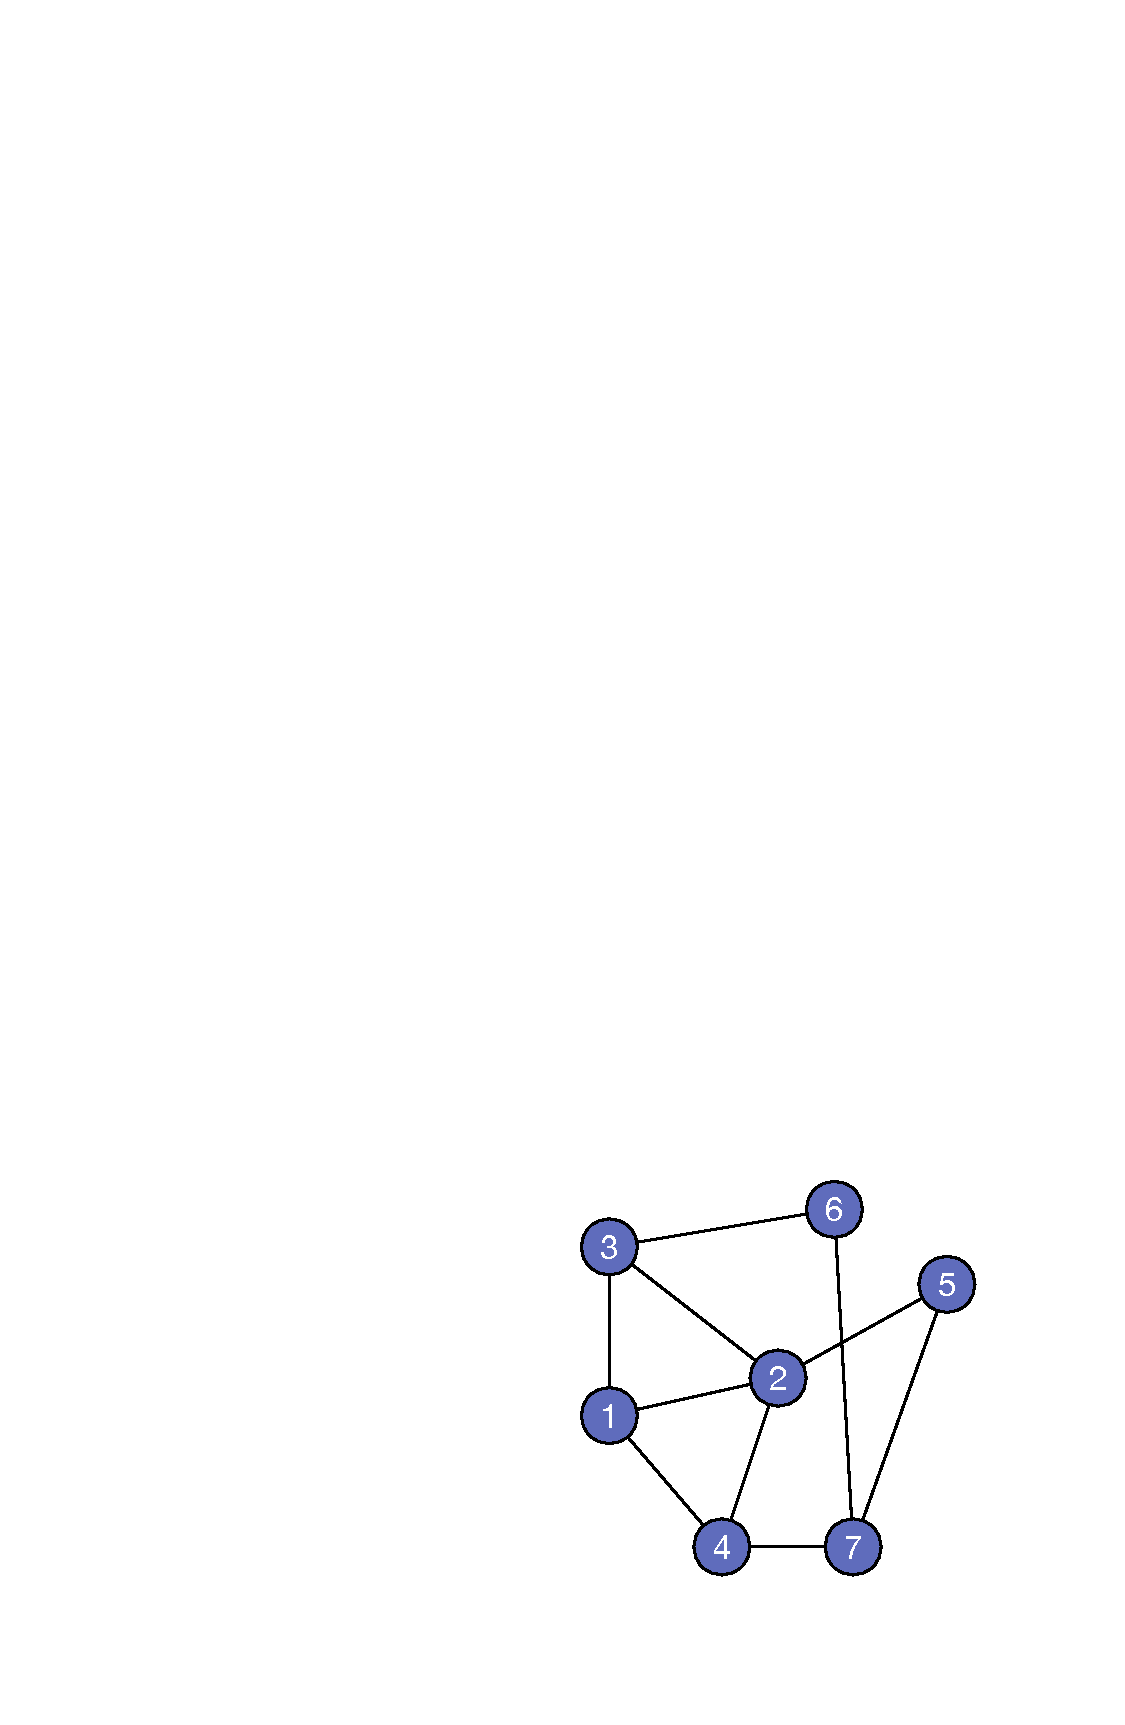
\includegraphics[scale=0.3]{CCTA}
    \caption{Distributed system with fault detection system embedded in agent 1.}
    \label{fig:CCTA}
\end{figure}
We provide an example to illustrate our approach. The system we consider is shown in Figure \ref{fig:CCTA} and is assumed to be under consensus using (\ref{eq:consensysDynSingle}) with the following Laplacian matrix:
\begingroup\makeatletter\def\f@size{5}\check@mathfonts
\def\maketag@@@#1{\hbox{\m@th\large\normalfont#1}}%
\begin{align*}
-\cL = \left [\begin{array}{ccccccc}
 -3&	1&     1&     1&     0&     0&     0 \\
 1&    -4&     1&     1&     1&     0&     0 \\
     1&     1&    -3&     0&     0&     1&     0 \\
     1&     1&     0&    -3&     0&     0&     1 \\
     0&     1&     0&     0&    -2&     0&     1 \\
     0&     0&     1&     0&     0&    -2&     1 \\
     0&     0&     0&     1&     1&     1&    -3
\end{array} \right ].
\end{align*}\endgroup
At $t=2$ sec we introduce fault signal $f(t) = 10u(t-2)$ where $u(t)$ is the step function. By definition \ref{def:Metz} this system is a positive system and we may design a positive residual generator to be embedded in agent 1. This agent's residual generator will be monitoring for faults in agents 2, 3 and 4. However, our design will choose to make the PUIO insensitive to faults from agent 3, therefore we will only be able to detect faults in agents 2 and 4. A separate UIO can be used to detect faults in agent 3. The PUIO for agent 1 is designed to be insensitive to all faults in agent 3 and sensitive to any fault imparted on to agents 2 and 4. %The parameter matrices are 
\begingroup\makeatletter\def\f@size{5}\check@mathfonts
\def\maketag@@@#1{\hbox{\m@th\large\normalfont#1}}%
\begin{align*}
F_1 &= \left [\begin{array}{ccccccc}
 -3&    0.87&    0.91&    0.49&         0&         0&         0 \\
    1&   -4.16&  0.81&    0.95&    1&         0&         0 \\
    1&    0.80&   -3.18&    0.02&         0&    1&         0\\
         0&    0.95&    0.01&   -3.35&         0&         0&         0\\
         0&    0.88&   -0.10&    0.01&   -2&         0&    1\\
         0&   -0.09&    0.88&    0.02&         0&   -2&    1\\
         0&   -0.11&   -0.07&    0.54&    1&    1&   -3\
\end{array} \right ],\\
G_1 &= \left [\begin{array}{ccccccc}
  0.13&    0.09&    1\\
    0.16&    0.18&    1\\
    0.19&    0.18&         0\\
   -0.94&   -0.01&         0\\
    0.11&    0.10&         0\\
    0.08&    0.11&         0\\
    0.11&    0.07&    1\\
\end{array} \right ]
\end{align*}\endgroup
$T_1 \in \R^{7 \times 7}$ identity matrix with $T_{1_{4,4}}=0$, $N \in \R^{7 \times 4}$ with only $n_{4,3} = 1$. 
As  shown in figure \ref{fig:faultAgent4}, the residual generator for D-PUIO is able to exceed the threshold and detect the fault in agent 4. Furthermore, as shown in figure \ref{fig:faultEstim}, the estimate of the fault signal $\hat{f}(t)$ is much better using D-PUIO.  
% \begin{figure}
%     \centering
%     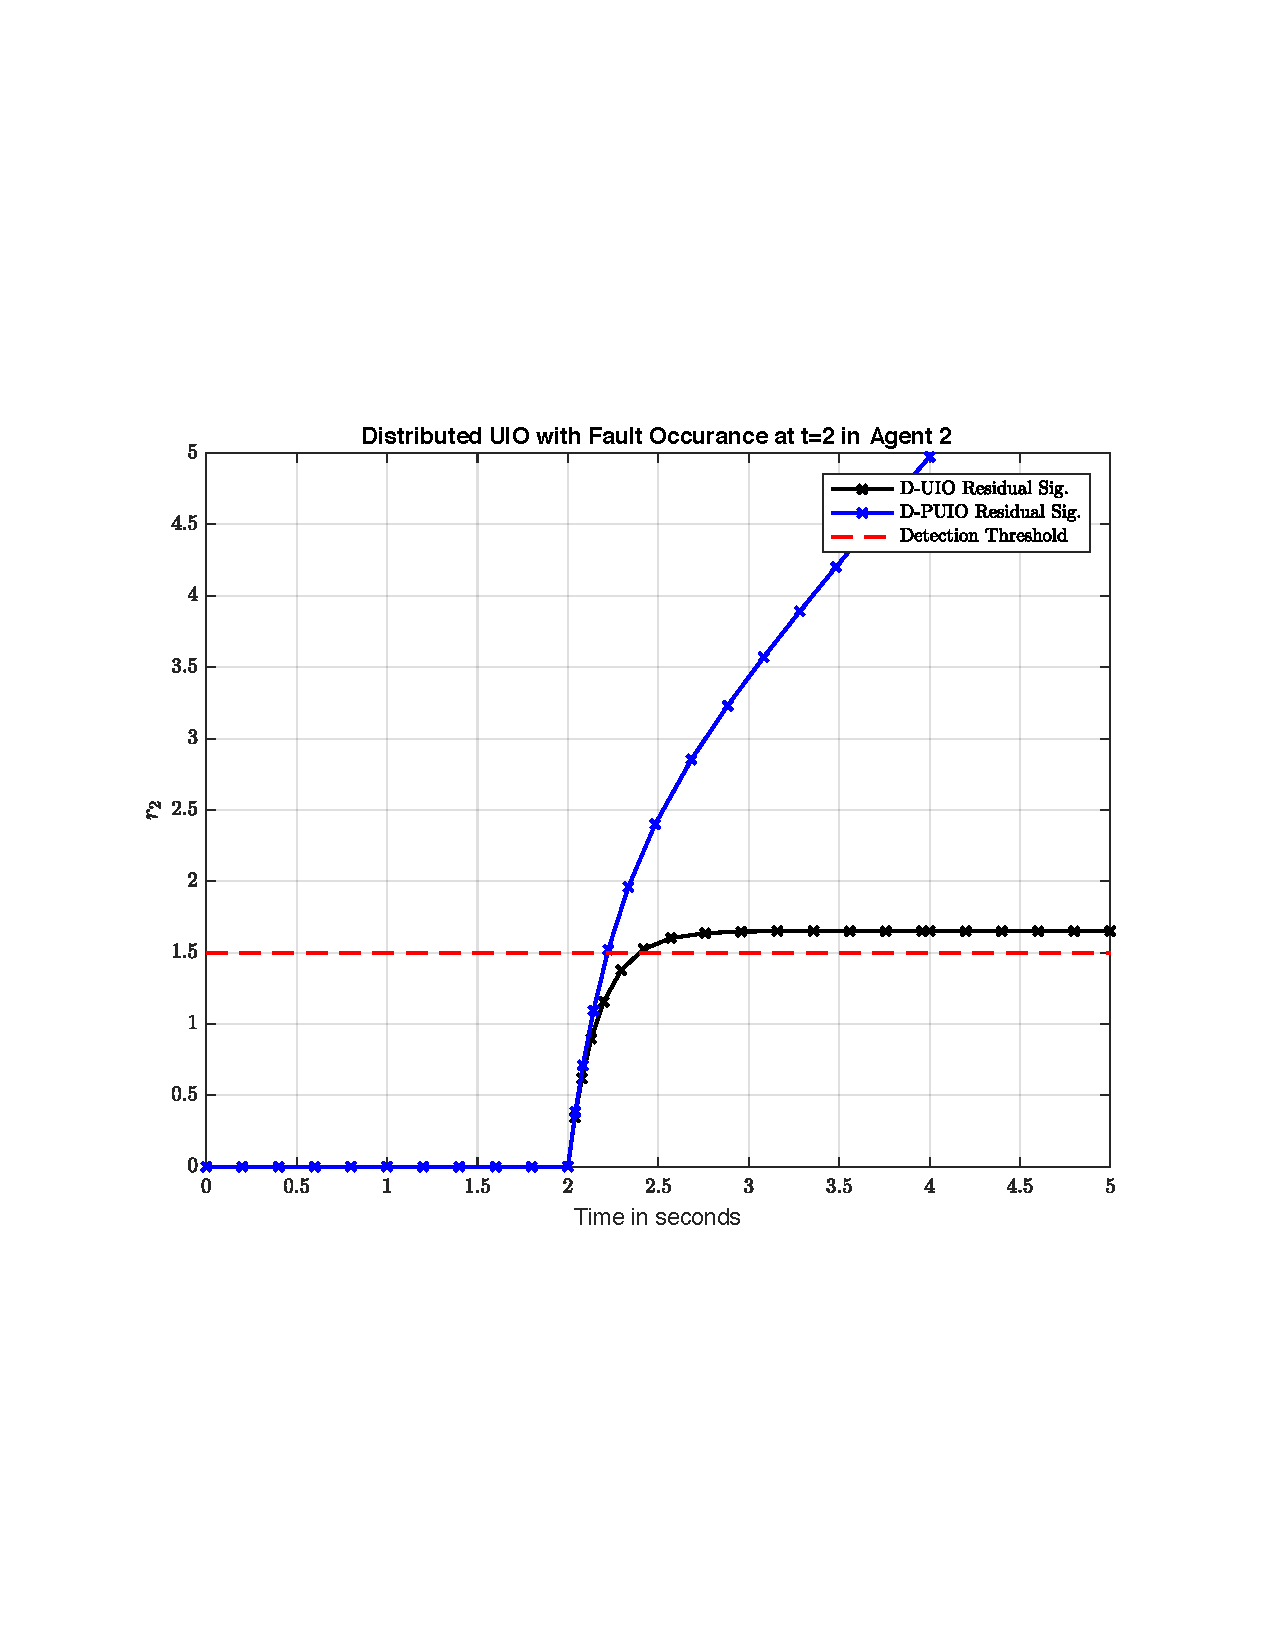
\includegraphics[scale=0.5]{faultAgent2}
%     \caption{A time series plot of the residual generator signal for D-UIO (black) and D-PUIO (blue). The fault occurs in Agent 2 at $t=2$ seconds. A threshold value of $1.5$ (red) was selected as the fault detection threshold that must be exceeded in order for the fault detection system to declare a fault in Agent 2. As shown in the figure, the time-to-detection, \ie the time interval between fault occurrence and fault detection is slightly better in D-PUIO. The time-to-detection was measured to be $\Delta T = 0. 27$ seconds for D-UIO and $\Delta T = 0.16$ seconds for D-PUIO.}
%     \label{fig:faultAgent2}
% \end{figure}

 \begin{figure}
    \centering
    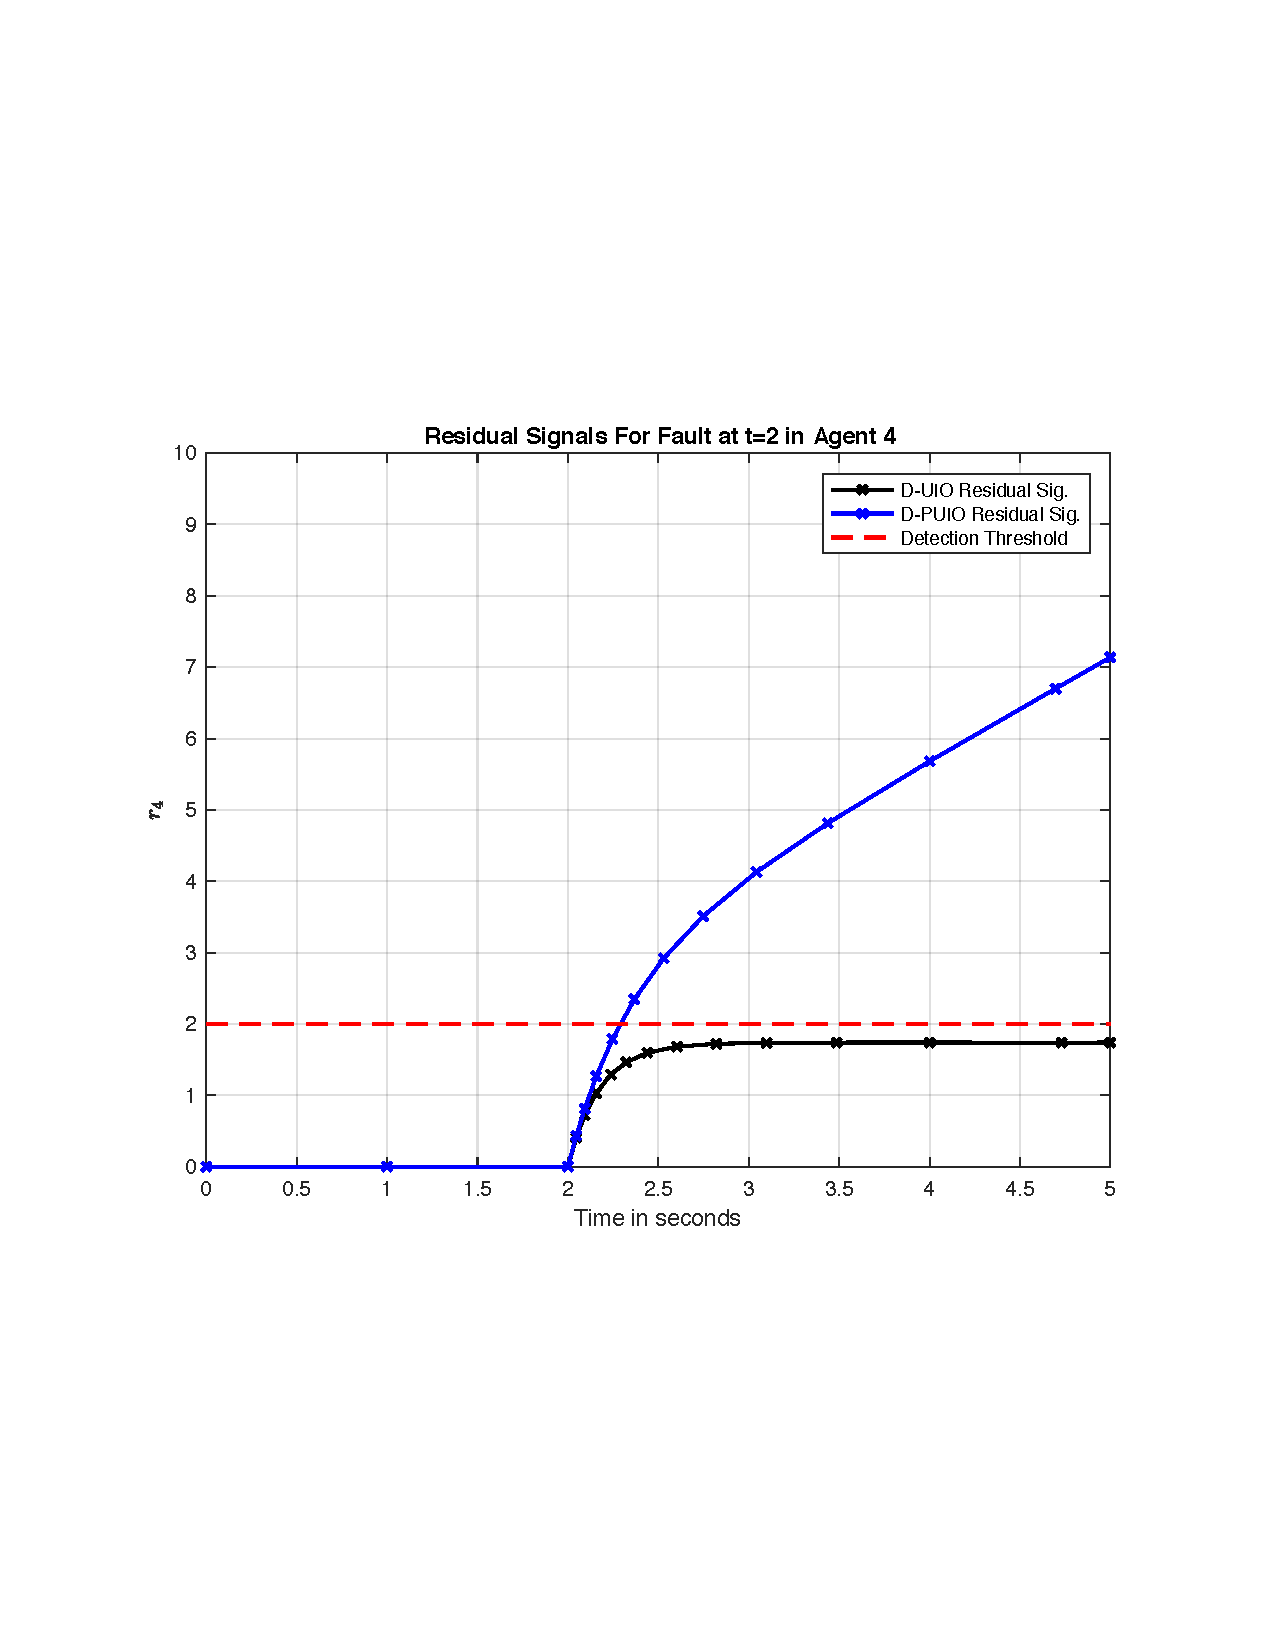
\includegraphics[scale=0.3]{residualSignalsAgent4}
    \caption{A time series plot of the residual generator signal for D-UIO (black) and D-PUIO (blue). The fault occurs in Agent 4 at $t=2$ seconds. A threshold value of $2.0$ (red) was selected as the fault detection threshold that must be exceeded in order for the fault detection system to declare a fault in Agent 4. As shown in the figure, the time-to-detection, \ie the time interval between fault occurrence and fault detection is $\Delta T = 0.22$ seconds in D-PUIO. The D-UIO observer does not reach this value and consequently does not trigger the fault detection system.}
    \label{fig:faultAgent4}
\end{figure}
 \begin{figure}
    \centering
    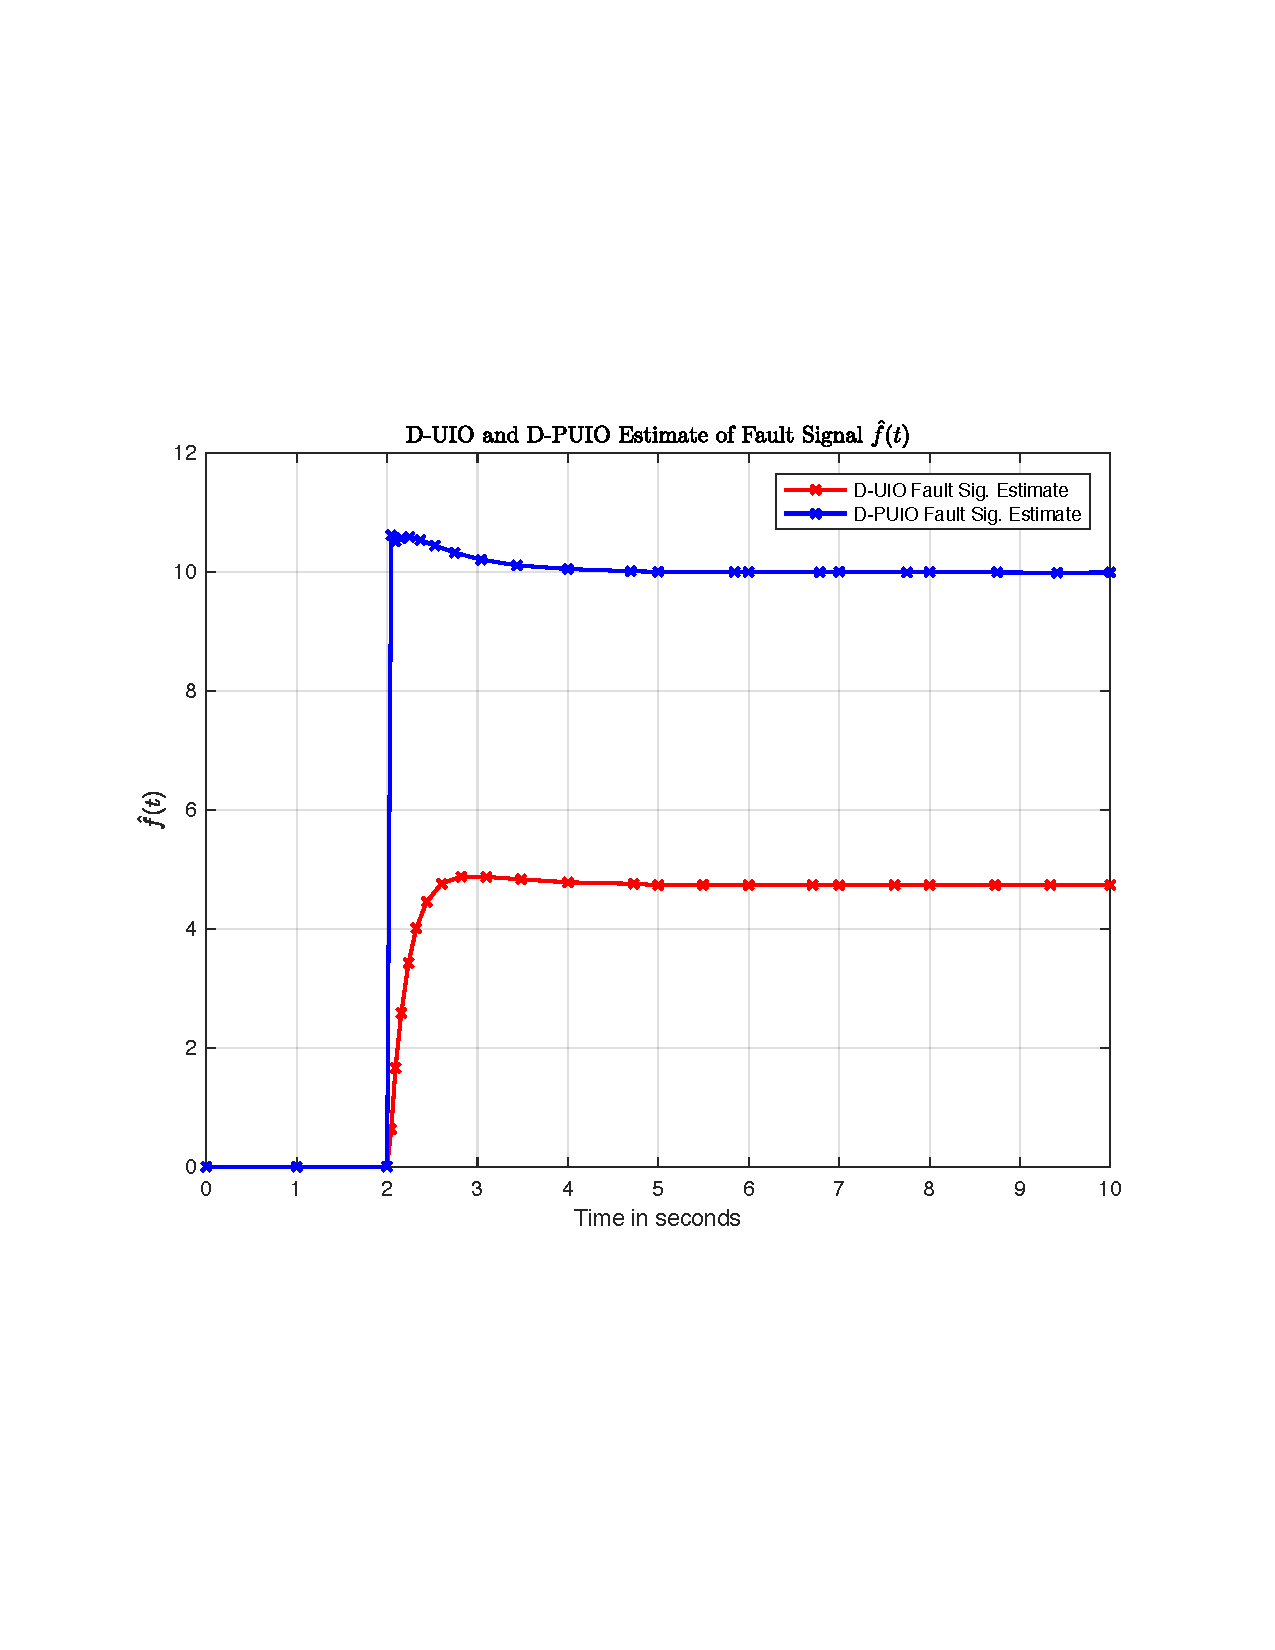
\includegraphics[scale=0.3]{faultEstim}
    \caption{Estimates of the fault signal $\hat{f}(t)$ with D-UIO (red) and D-PUIO (blue). The fault signal was introduced at 2 seconds as $f(t) =10u(t-2)$. As can be seen, the fault estimate produced by D-PUIO converges to the correct value. }
    \label{fig:faultEstim}
\end{figure}
%%%%%%%%%%%%%%%%%%%%%%%%%%%%%%%%%%%%%%%%%%%%%%%%%%%%%%%%%%%%%%%%%%%%%%%%%%%%%%%%
\section{Conclusion} \label{sec:con}
In this paper, we considered robust fault detection in distributed systems with first and second order agent models. We showed that a ubiquitous class of consensus protocols leads to collective dynamics that lie in a nonnegative invariant set. Based on this, we derived LMI conditions for residual generators to sense faults in the nonnegative invariant set. We highlighted the advantages of our approach through an illustrative example.

\bibliography{Zotero.bib}
\bibliographystyle{IEEEtran}
\end{document}
